\documentclass[10pt,a4paper]{article} 
\usepackage[utf8]{inputenc} 
\usepackage[T1]{fontenc} 
\usepackage[french]{babel} 
\usepackage{supertabular}  %Nécessaire pour les longs tableaux
\usepackage[top=2.2cm, bottom=2.5cm,
	    right=2.5cm, left=2.5cm]{geometry}  %Mise en page 
\usepackage{amsmath}  %Nécessaire pour les maths 
\usepackage{amssymb}  %Nécessaire pour les maths 
\usepackage{stmaryrd}  %Utilisation des double crochets 
%\usepackage{pifont}  %Utilisation des chiffres entourés 
\usepackage{graphicx}  %Introduction d images 
\usepackage{epstopdf}  %Utilisation des images .eps 
\usepackage{amsthm}  %Nécessaire pour créer des théorèmes 
%\usepackage{algorithmic}  %Nécessaire pour écrire des algorithmes 
%\usepackage{algorithm}  %Idem 
\usepackage{bbold}  %Nécessaire pour pouvoir écrire des indicatrices 
\usepackage{hyperref}  %Nécessaire pour écrire des liens externes 
\usepackage{array}  %Nécessaire pour faire des tableaux 
\usepackage{tabularx}  %Nécessaire pour faire de longs tableaux 
\usepackage{caption}  %Nécesaire pour mettre des titres aux tableaux (tabular) 
\usepackage{color}  % Nécessaire pour écrire en couleur 
\usepackage{float}  % Pour l'option [H] de \begin{figure}
\newtheorem{thm}{Théorème} 
\newtheorem{mydef}{Définition}
\newtheorem{prop}{Proposition} 
\newtheorem{lemma}{Lemme}

\newcommand{\hmm}{\textsc{HMM}}
\newcommand{\mcmc}{\textsc{MCMC}}
\newcommand{\fhmm}{\textsc{Factorial HMM}}
\newcommand{\Estep}{\textsc{E-step}}
\newcommand{\Mstep}{\textsc{M-step}}
\newcommand{\EM}{\textsc{EM}}
\newcommand{\meanfield}{\textsc{mean-field}}
\newcommand{\structmeanfield}{\textsc{structured mean-field}}

\title{MVA, Projet PGM : Rapport\\
  Factorial HMM}
\author{Théis \textsc{Bazin} \and Valentin \textsc{De Bortoli} \and Élie 
\textsc{Michel}}

\begin{document}

\maketitle

\section{Présentation du modèle}
\subsection{Comparaison avec HMM}
Le but de ce rapport est de présenter le modèle \emph{Factorial HMM}, extension 
du modèle \hmm, \emph{Hidden Markov Model}. Ce dernier suppose qu'une variable 
aléatoire cachée, dont l'évolution temporelle est régie par une chaine de variables
cachées, est à l'origine d'une observation. Le modèle que l'on se 
propose d'étudier ici met en parallèle $M$ chaînes \footnote{Malgré la 
similitude avec $M$ chaînes de Markov indépendantes et homogènes, il est incorrect
d'utiliser cette terminologie ici puisque les chaînes sont couplées via les variables
d'observation} de variables cachées
 qui sont à l'origine d'une observation. Ce modèle décrit bien
des situations d'évolution temporelle dans lesquelles plusieurs facteurs 
indépendants entrent en jeu.
L'espace d'état de chaque variable cachée est  supposé être le même et est fini
de cardinal $K$.

On pourrait tenter de regrouper les variables cachées en une seule variable et
considérer le modèle  \hmm{} connu.
Ce modèle n'est pas satisfaisant pour deux raisons :

\begin{itemize}
  \item l'espace d'état de cette unique variable cachée est alors de cardinal 
    $K^M$, on arrive rapidement aux limites numériques des ordinateurs.
  \item l'information sur l'indépendance des variables cachées est perdue.
\end{itemize}

Ces deux remarques justifient l'intérêt et la complexité de \fhmm.

\subsection{Graphe associé et inférence} 
Compte tenu de la proximité entre le modèle \fhmm{} et \hmm{} il est naturel de 
se poser la question de l'inférence et de la possibilité de construire un
algorithme pour apprendre les paramètres du modèle.
Dans ce but, on présente le graphe de \fhmm.
Ce graphe permet de mettre à nouveau en évidence la complexité du nouveau 
modèle.

\begin{figure}[H]
  \centering
  \begin{minipage}{.46\linewidth}
    \centering
      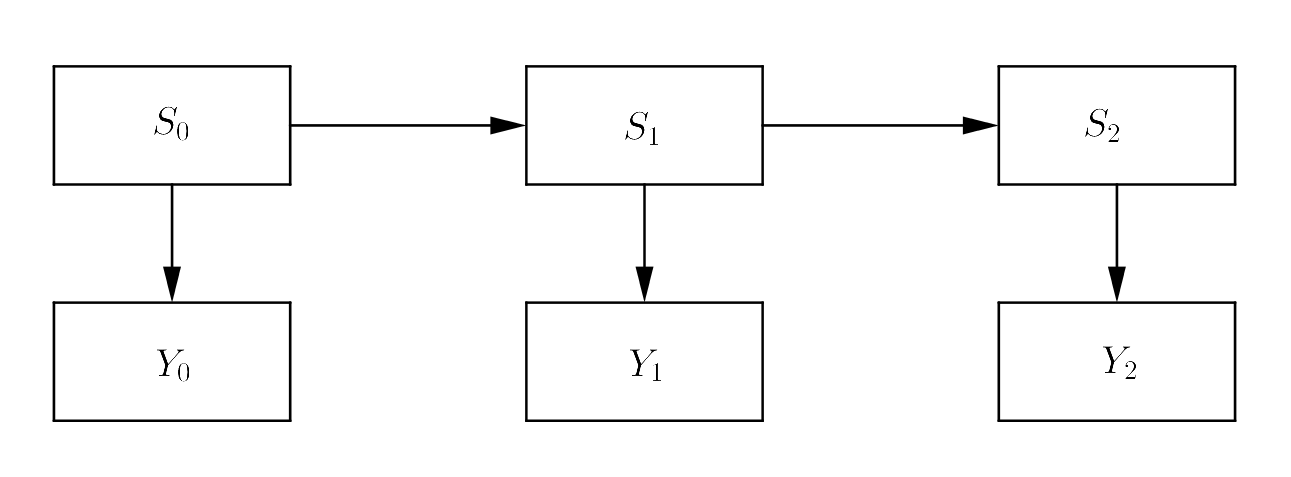
\includegraphics[scale=0.2]{../resources/pictures/graph1.png}
      \caption{Modèle \hmm}
  \end{minipage}
  \begin{minipage}{.46\linewidth}
    \centering
      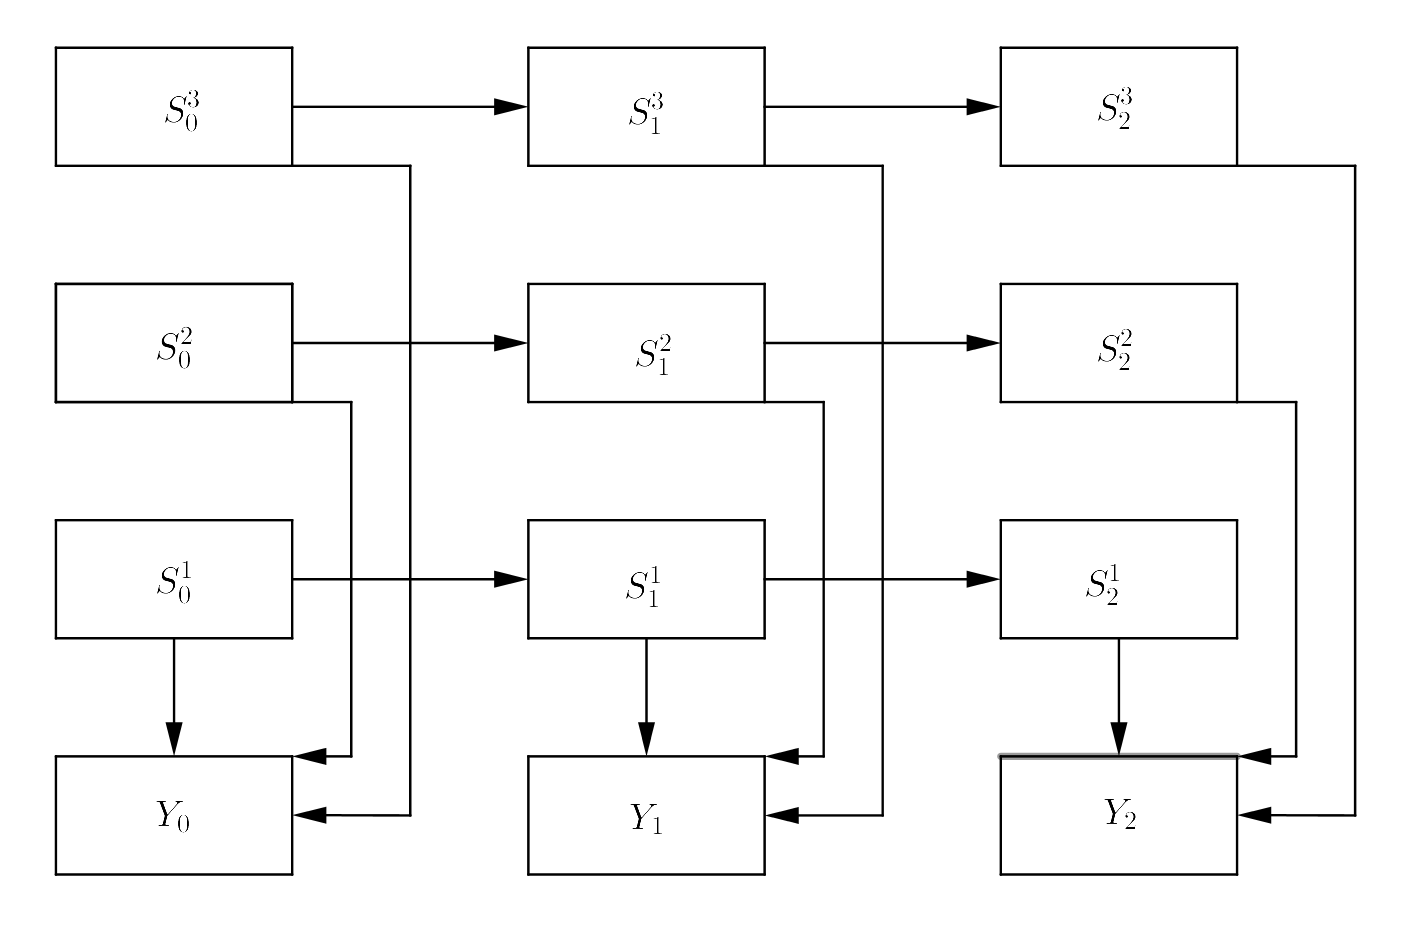
\includegraphics[scale=0.2]{../resources/pictures/graph2.png}
      \caption{Modèle \fhmm}
  \end{minipage}
\end{figure}

Dans le cas de \fhmm{} on perd la structure d'arbre.
Néanmoins, on peut développer un algorithme semblable à celui développé dans 
\hmm{} qui permet de calculer exactement les marginales des probabilités se 
factorisant sur le graphe.
Il est alors possible de résoudre exactement \Estep{} dans un algorithme 
\emph{Expectation-Maximization}, \EM. Néanmoins, cet algorithme exact n'est pas 
satisfaisant dès lors que le nombre de chaînes devient important.
On se tourne alors vers trois méthodes d'approximation :
\begin{itemize}
  \item l'échantillonnage de Gibbs (\emph{Gibbs sampling}),
  \item \textit{mean-fields},
  \item \textit{structured mean-fields}.
\end{itemize}

Toutes ces méthodes ont été implémentées et testées sur des données de synthèse.

\subsection{Notations}

On reporte dans le \autoref{tab:notations} les notations qui seront utilisées
dans toute la suite de notre rapport.

\begin{table}[hpbt]

\begin{center}
  \begin{tabular}{|c|c|}
  \hline
  $T \in \mathbb{N}$ & temps de la dernière observation \\ \hline
  $M \in \mathbb{N}^*$ & nombre de chaînes de Markov \\ \hline
  $\Delta_K=\lbrace X \in \lbrace0,1\rbrace^K, \ 
  \underset{k=1}{\overset{K}{\sum}}X_k=1\rbrace$ & espace d'état des variables 
  cachées \\ \hline
  $D \in \mathbb{N}^*$ & dimension des variables observées \\ \hline
  $(\Pi_{k}^m)_{(m,k) \in \llbracket 1,M \rrbracket \times \llbracket 1,K 
  \rrbracket} \in [0,1]^{MK}$ & mesures de probabilité initiales pour chaque 
  chaîne \\ \hline
  $(A_{k_1,k_2}^m)_{(m,k_1,k_2) \in \llbracket 1,M \rrbracket \times \llbracket 
  1,K \rrbracket^2} \in [0,1]^{MK^2}$ & matrices de transition pour chaque chaîne 
   \\ \hline
  $C \in \mathcal{S}_D^{++}(\mathbb{R})$ & matrice de covariance \\ \hline
  $(W_{x,k}^m)_{(m,x,k) \in \llbracket 1,M \rrbracket \times \llbracket 1,D 
  \rrbracket \times \llbracket 1,K \rrbracket} \in \mathbb{R}^{MDK}$ & matrices 
  d'influence des variables cachées sur les variables observées \\ \hline
  $(S_t^m)_{(m,t) \in \llbracket 1,M \rrbracket \times \llbracket 0,T \rrbracket 
  } \in \Delta_K^{(T+1)\times M}$ & variables cachées \\ \hline
  $(Y_t)_{t \in \llbracket 0,T \rrbracket} \in \mathbb{R}^D$ & variables 
  observées \\ \hline
  \end{tabular}
  \caption{Notations\label{tab:notations}}
\end{center}
\end{table}

Les différentes contraintes (sommation à 1) sur les mesures de probabilité 
n'ont pas été rappelées ici. Pour plus de simplicité on notera $Y_{(t)}$ le 
vecteur $(Y_t)_{t \in \llbracket 0,T \rrbracket}$, $Y_{(-t)}$ le vecteur 
$(Y_{t})_{t \in \llbracket 0,T \rrbracket\backslash \lbrace t \rbrace}$, 
$Y_{(t_1,t_2)}$ le vecteur $(Y_t)_{t \in \llbracket t_1,t_2 \rrbracket}$. Ces 
notations s'étendent aux variables cachées. Enfin on notera $\theta=(\Pi, 
A,C,W)$ le vecteur de paramètres. Si il n'y pas d'ambiguïté la dépendance 
par rapport à $\theta$ est sous-entendue
\section{Le problème d'inférence et l'algorithme EM}
\subsection{Algorithme EM}
Soit $p$ une mesure de probabilité qui se factorise selon \fhmm. On a alors :
\begin{multline}
p(S_{(t)}^{(m)},Y_{(t)} \vert 
\theta)=\underset{m=1}{\overset{M}{\prod}}\underset{k=1}{\overset{K}{\prod}}
(\Pi_k^m)^{(S_0^m)_k}\underset{t=1}{\overset{T}{\prod}}\underset{m=1}{\overset{M
}{\prod}}\underset{k_1=1}{\overset{K}{\prod}}\underset{k_2=1}{\overset{K}{\prod}
}(A_{k_1,k_2}^m)^{(S_t^m)_{k_2}(S_{t-1}^m)_{k_1}}\\ 
\underset{t=0}{\overset{T}{\prod}}\frac{1}{(2\pi)^{D/2}}\frac{1}{\vert C  
\vert^{1/2}}\exp\left(-1/2 {}^t\left(Y_t- \underset{m=1}{\overset{M}{\sum}}W^m 
S_t^m \right)C^{-1} \left(Y_t- \underset{m=1}{\overset{M}{\sum}}W^m S_t^m 
\right)\right) \label{jointprob}
\end{multline}
De manière analogue au cas \hmm{} ou \textsc{Gaussian mixture} il n'est pas 
facile de calculer $p(Y_{(t)})$. L'algorithme \EM{} est une méthode itérative 
qui 
permet de considérer seulement la probabilité jointe \ref{jointprob} dont la 
forme est facile à manipuler. L'idée est la suivante :
\begin{equation}
\begin{aligned}
p(Y_{(t)})&=\int_{S_{(t)}^{(m)}}p(S_{(t)}^{(m)},Y_{(t)}) \\
&=\int_{S_{(t)}^{(m)}}\frac{p(S_{(t)}^{(m)},Y_{(t)})}{q(S_{(t)}^{(m)})}q(S_{(t)}
^{(m)}) \\
&=\mathbb{E}_q\left(p(S_{(t)}^{(m)},Y_{(t)}) \right)
\end{aligned}
\end{equation}
Si on considère la log-vraisemblance on peut utiliser l'inégalité de Jensen et 
on obtient :
\begin{equation}
\begin{aligned}
l(Y_{(t)},\theta)&=\log(p(Y_{(t)}) \\
&=\log\left( \mathbb{E}_q\left( 
\frac{p(S_{(t)}^{(m)},Y_{(t)})}{q(S_{(t)}^{(m)})} \right) \right)
&\ge \mathcal{L}(Y_{(t)},\theta,q)
\end{aligned}
\end{equation}
Avec $\mathcal{L}(Y_{(t)},\theta,q)=\mathbb{E}_q \log \left( p(S_{(t)}^{(m)}, 
Y_{(t)})\right)+H(q)$ où $H(q)$ est l'entropie de $q$. Il s'agit alors de 
maximiser cette log-vraisemblance approchée en $q$ et en $\theta$. La 
maximisation à $\theta$ fixé implique 
\begin{equation}
\hat{q}=p(S_{(t)}^{(m)} \vert \theta,Y_{(t)}^{(m)})
\end{equation} 
Une autre conséquence est l'égalité suivante :
\begin{equation}
\mathcal{L}(Y_{(t)},\theta,\hat{q})=l(Y_{(t)},\theta) \label{increase}
\end{equation}
L'algorithme consiste à appliquer un algorithme de Gauss-Seidel avec 
contraintes sur la log-vraisemblance approchée, les deux variables considérées 
étant $q$ \footnote{$q$ peut être vue comme une mesure de probabilité mais d'un 
point de vue optimisation on considère $q$ comme une variable de $[0,1]^{K^M}$} 
et $\theta$. On distingue ainsi deux étapes :
\begin{itemize}
\item \Estep{} : $q_{n+1}=p(S_{(t)}^{(m)} \vert \theta_n,Y_{(t)}^{(m)})$
\item \Mstep{} : maximisation de $\mathbb{E}_{q_n} \left( \log \left( 
p(S_{(t)}^{(m)}, Y_{(t)}  \vert  \theta )\right) \right)$
\end{itemize}
Les conditions initiales n'ont pas été discutées ici. Néanmoins elles jouent un 
rôle crucial dans cet algorithme au comportement très local. En effet, très peu 
de résultats assurent la convergence théorique de cet algorithme vers un 
maximum local. Dans \cite{wu1983convergence}, les auteurs montrent que sous 
certaines conditions on a l'assurance de la convergence vers un point 
stationnaire. Les conditions de maximalité sont plus dures à obtenir. Il est 
cependant important de remarquer que \ref{increase} assure une croissance de la 
log-vraisemblance à chaque étape de l'algorithme.

\subsection{M-step}

On détaille désormais l'étape \Mstep{} de notre algorithme.
On rappelle qu'il s'agit de maximiser
$\mathcal{L}_{approx}(\theta)=\mathbb{E}_{q_n}
\left( \log \left( p(S_{(t)}^{(m)},Y_{(t)}\vert \theta)\right)\right)$.
La maximisation selon
$(\Pi_{k}^m)_{(m,k) \in
\llbracket 1,M \rrbracket \times \llbracket 1,K \rrbracket}$
(respectivement selon
$(A_{k_1,k_2}^m)_{(m,k_1,k_2) \in
\llbracket 1,M \rrbracket \times \llbracket 1,K \rrbracket^2}$) pouvant se faire 
indépendamment des autres variables, on obtient après utilisation des 
multiplicateurs de Lagrange\footnote{Le fait que l'on travaille sur des 
ouverts, i.e $\Pi_{k}^m$ et $A_{k_1,k_2}^m$ ne s'annulent jamais, n'est pas 
détaillé ici. Cette propriété est issue de la divergence du logarithme en $0$} :

\begin{equation}
  \widehat{\Pi_k^m}=q_{n}((S_0^m)_k=1)
\end{equation}

De même on obtient :

\begin{equation}
  \widehat{A_{k_1,k_2}^m}=\frac{\underset{t=1}{\overset{T}{\sum}}q_n((S_{t-1}^m)_{
  k_1}=1,(S_t^m)_{k_2}=1)}{\underset{t=1}{\overset{T}{\sum}}q_n((S_{t-1}^m)_{k_1}
  =1)}
\end{equation}

  Pour la suite, on note $W \in \mathcal{M}_{DM,K}(\mathbb{R})$ la matrice 
obtenue en concaténant les matrices $(W_m)_{m \in \llbracket 1,M \rrbracket}$. 
De la même manière on note $S_t$ le vecteur obtenu en concaténant tous les 
vecteurs $(S_t^m)_{m \in \llbracket 1,M \rrbracket}$.
Il s'agit alors de maximiser en $(W,C)$ la fonction suivante 
\[ \mathcal{L}'(W,C)=\mathbb{E}_{q_n}\left(-\frac{T+1}{2} \log(\vert C \vert) 
-\frac{1}{2} {}^t\left(Y_t-WS_t \right)C^{-1} \left( Y_t-WS_t\right)\right) \].
Cette étude est classique (maximisation des paramètres pour la 
log-vraisemblance d'une gaussienne) et les calculs ont déjà été effectués à 
plusieurs reprises.
On rappelle simplement que la maximisation se fait d'abord sur $W$, l'argument
maximum ne dépendant pas de $C$ on peut facilement réinjecter
$\widehat{W}$ dans $\mathcal{L}'(\widehat{W},C)$ et optimiser selon
$C$\footnote{En réalité on optimise selon $C^{-1}$ qui donne une 
expression plus facile à manipuler}.
On obtient les expressions suivantes :

\begin{equation}
  \widehat{W}=\left( \underset{t=0}{\overset{T}{\sum}} Y_t \times 
  \mathbb{E}_{q_n}({}^tS_t) \right) \left( \underset{t=0}{\overset{T}{\sum}} 
  \mathbb{E}_{q_n}\left( S_t {}^t S_t\right)\right)^+
\end{equation}
Où $M^+$ est la pseudo-inverse de Moore-Penrose. On a ici utilisé le fait que 
la pseudo-inverse de Moore-Penrose donne une solution au problème des moindres 
carrés \cite{ben2003generalized}. La maximisation selon $C^{-1}$ donne :
\begin{equation}
\widehat{C}=\frac{1}{T+1}\underset{t=0}{\overset{T}{\sum}}Y_t 
{}^tY_t-\frac{1}{T+1}\underset{t=0}{\overset{T}{\sum}}\underset{m=1}{\overset{M}
{\sum}}W^m\mathbb{E}_{q_n}(S_t^m){}^t Y_t
\end{equation}
On remarque que les mises à jour données par \Mstep{} dépendent de \Estep{} 
uniquement pour le calcul de trois quantités :
\begin{itemize}
\item $\forall (t,m) \in \llbracket 0, T\rrbracket \times \llbracket 1,M 
\rrbracket, \ \mathbb{E}_{q_n}(S_t^m) $
\item $\forall (t,m_1,m_2) \in \llbracket 0, T\rrbracket \times \llbracket 
1,M\rrbracket^2, \ \mathbb{E}_{q_n}(S_t^{m_1}S_t^{m_2}) $
\item $\forall t \in \llbracket 1,T \rrbracket \times \llbracket 1,M 
\rrbracket, \ \mathbb{E}_{q_n}(S_{t-1}^mS_t^{m})$
\end{itemize}
On rappelle que les multiplications considérées ici le sont élément par 
élément. Il s'agit donc de calculer ces trois quantités afin de pouvoir les 
réinjecter dans \Mstep. Pour cela, on considère tout d'abord une méthode
d'inférence \emph{exacte}, deux méthodes d'inférences \emph{variationnelles} et
une méthode d'\emph{échantillonnage}.

\section{E-step}

\subsection{Inférence exacte}

Pour présenter cet algorithme il est bon d'avoir à l'esprit les calculs 
effectués lors de la récurrence alpha-beta de \hmm. Les calculs sont très 
semblables, néanmoins le problème est ici plus complexe puisque l'on n'a non pas
une chaîne de Markov mais $M$. On pose :
\begin{equation}
\left\lbrace
\begin{aligned}
&\alpha_t=p(S_t^{1},\dots,S_t^{M},Y_{(1,t)}\vert \theta) \\
&\forall m \in \llbracket 1,M \rrbracket, \ \alpha_t^m=p(S_{t-1}^1, \dots, 
S_{t-1}^m,S_{t}^{m+1}, \dots, S_{t}^M, Y_{(1,t-1)} \vert \theta) \\
&\beta_t=p(Y_{(t+1,T)} \vert S_t^1, \dots,S_t^M, \theta) \\
&\forall m \in \llbracket 1,M \rrbracket, \ \beta_t^m=p(Y_{(t,T)} \vert S_t^1, 
\dots, S_t^m,S_{t-1}^{m+1}, \dots, S_{t-1}^M, \theta)
\end{aligned}
\right.
\end{equation}
On remarque que :
\begin{equation}
\left\lbrace 
\begin{aligned}
&\forall t \in \llbracket 1,T \rrbracket, \ \alpha_{t-1}=\alpha_{t}^M  \\
&\forall t \in \llbracket 0,T \rrbracket, \ \beta_{t}=\beta_{t}^0
\end{aligned}
\right.
\end{equation}
Quatre autres équations permettent de compléter la récurrence :
\begin{equation}
\left\lbrace
\begin{aligned}
&\alpha_t=p(Y_t \vert S_t^{(m)}, \theta)\alpha_t^0 \\
&\forall m \in \llbracket 0,M-1 \rrbracket, \ 
\alpha_t^m=\underset{S_{t-1}^{m+1}}{\sum}p(S_t^{m+1} \vert S_{t-1}^{m+1}, 
\theta) \alpha_t^{m+1} \\
&\beta_{t-1}^M=P( Y_t \ \vert S_t^{(m)},\theta) \beta_t \\
&\forall m \in \llbracket 0, M-1 \rrbracket, \ 
\beta_t^{m}=\underset{S_{t+1}^{m+1}}{\sum}p(S_{t+1}^{m+1} \vert S_{t}^{(m+1)}, 
\theta) \beta_{t}^{m+1}
\end{aligned}
\right.
\end{equation}
On obtient le schéma suivant :
\begin{figure}[H]
\centering
\begin{minipage}{.46\linewidth}
\centering
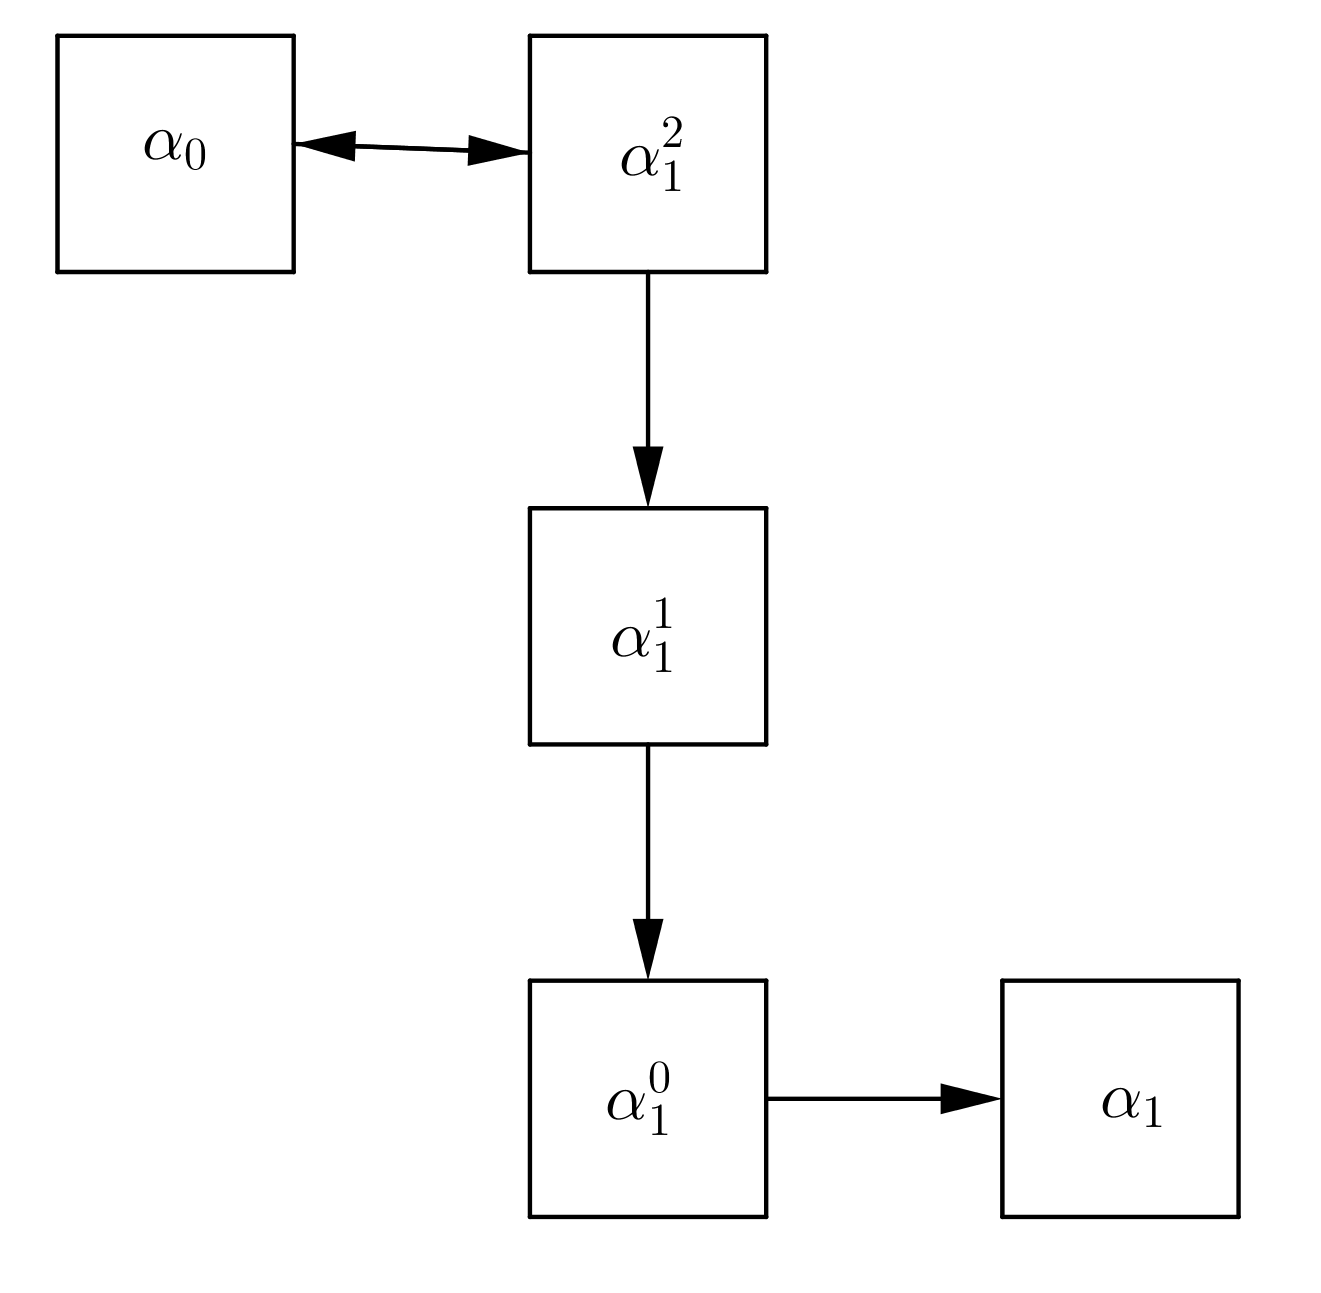
\includegraphics[scale=0.2]{../resources/pictures/graph3.png}
\caption{Récurrence sur $\alpha$}
\end{minipage}
\begin{minipage}{.46\linewidth}
\centering
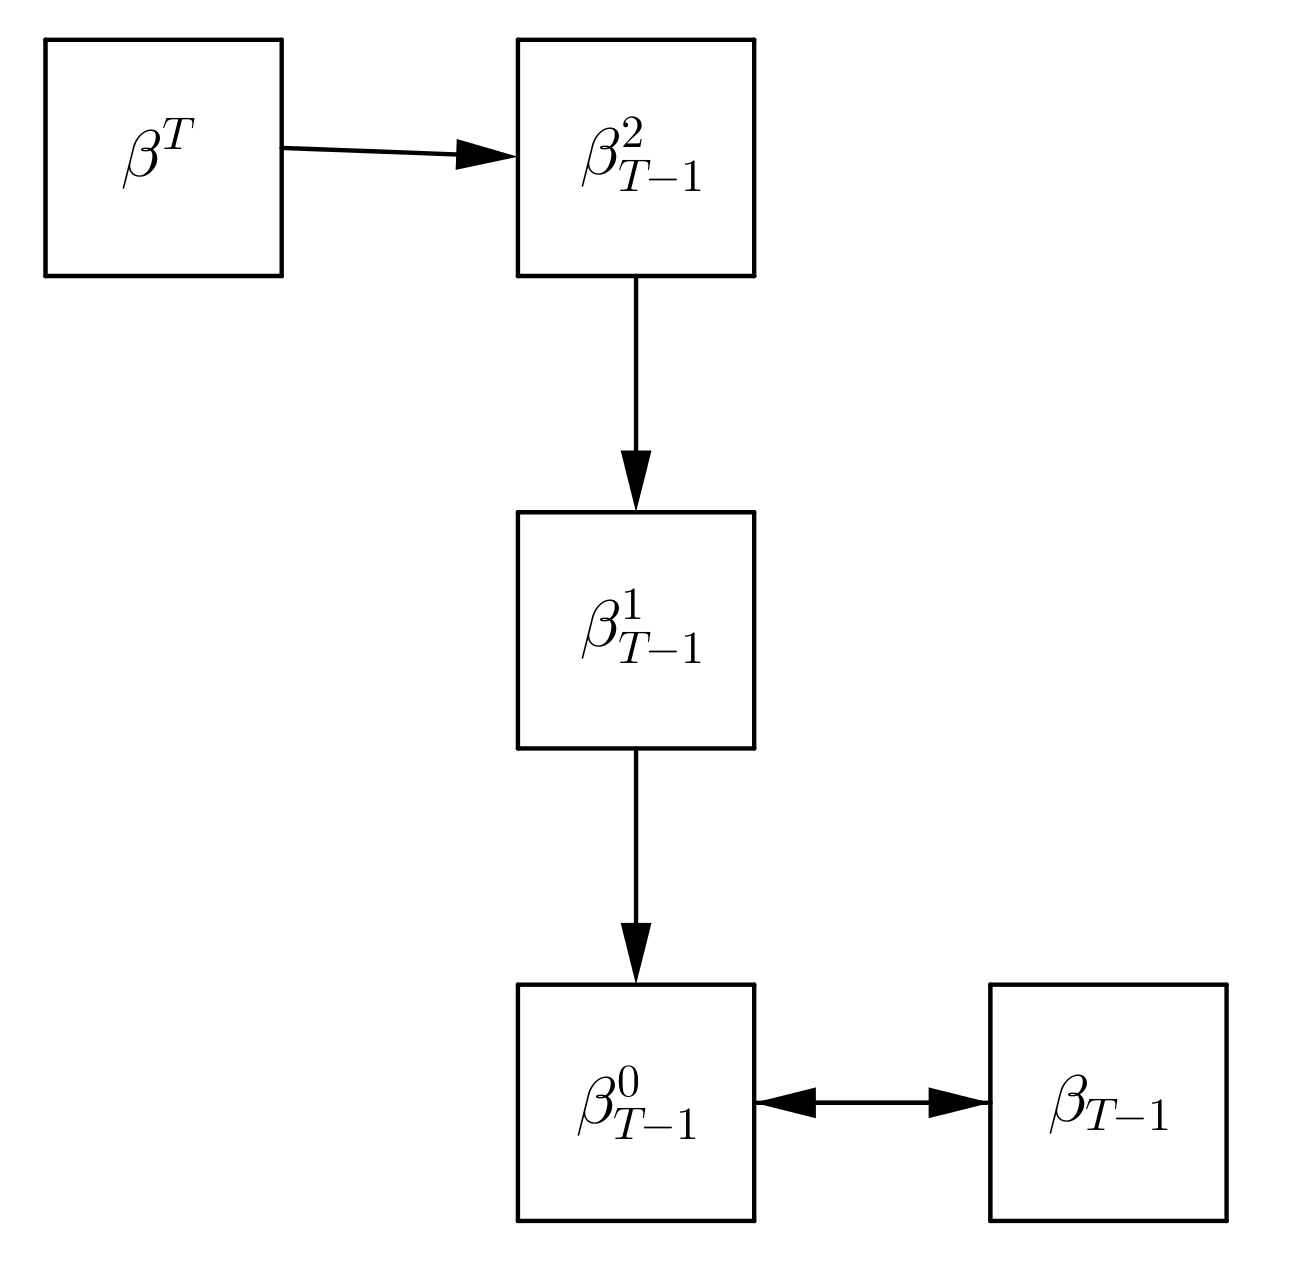
\includegraphics[scale=0.2]{../resources/pictures/graph4.png}
\caption{Récurrence sur $\beta$}
\end{minipage}
\end{figure}
On peut alors calculer $\gamma_t$ de la manière suivante :
\begin{equation}
\gamma_t=p(S_t \vert Y_{(t)}, \theta)= \frac{\alpha_t 
\beta_t}{\underset{S_t}{\sum} \alpha_t \beta_t}
\end{equation}
Il convient alors de calculer les trois quantités issues de \Mstep{} :
\begin{itemize}
\item $\mathbb{E}_{q_n}(S_t^m)= \underset{S_t^n, \ n \neq m}{\sum} \gamma_t$
\item $\mathbb{E}_{q_n}(S_t^{m_1}S_t^{m_2})= \underset{S_t^n, \ n \neq m_1, \ n 
\neq m_2}{\sum} \gamma_t$
\item $\mathbb{E}_{q_n}(S_{t-1}^mS_t^m)= \frac{\underset{S_{t-1}^n,S_t^r, \ n 
\neq m, \ r \neq m}{\sum}\alpha_{t-1} p(S_t \vert S_{t-1}) p(Y_t \vert S_t) 
\beta_t}{\underset{S_{t-1}, S_t}{\sum}\alpha_{t-1}p(S_t \vert S_{t-1})p(Y_t 
\vert S_t) \beta_t} $
\end{itemize}
Il est important de préciser que les formules données sont exactes seulement 
lorsqu'elles sont appliquées en un point. En effet, $\alpha_t, \beta_t, 
\gamma_t$ sont des éléments de $\mathbb{R}^{\llbracket 1,K \rrbracket^M}$. Pour 
plus de détails sur le sens de ces formules on renvoie à l'implémentation en 
Python de cet algorithme \href{url}{https://github.com/eliemichel/fHMM}.

\subsection{Échantillonnage de Gibbs}

L'inférence exacte peut être très couteuse en termes d'opérations (avec une
complexité temporelle en $\mathcal{O}(TMK^{M+1})$).
L'algorithme d'échantillonnage de Gibbs fournit, lui, un moyen d'échantillonner
approximativement selon $p(S_{(t)}^{(m)} \vert  Y_{(t)}, \theta)$ de
manière rapide.
En effet, l'échantillonnage de Gibbs peut être vu comme un cas particulier de
\emph{Monte Carlo Markov Chain}, pour laquelle la convergence en probabilité est
assurée.
Néanmoins, on ne possède pas d'information sur la vitesse de convergence de ces
algorithmes vers la probabilité voulue.

  Le choix des auteurs de \cite{ghahramani1997factorial} a été de ne pas prendre
en compte le temps de mise en route de l'échantillonneur de Gibbs
(\og{}\emph{burn-in period}\fg{}, durant laquelle les échantillons ne sont pas supposés
suivre la distribution de probabilité souhaitée) et de directement sélectionner
les premiers échantillons produits par l'algorithme.
Ce choix sera discuté par la suite.

On précise le déroulement de l'échantillonnage :
\begin{itemize}
  \item les différents états $S_{(t)}^{(m)}$ sont initialisés selon une loi 
    uniforme sur $\llbracket 1,K \rrbracket$,
  \item les états $S_0^{(m)}$ sont mis à jour de manière successive (d'abord 
    $S_0^1$ tiré selon $p(S_0^1 \vert Y_{0}, S_1^1, S_0^{(-1)}$, puis $S_0^2$ tiré 
    selon $p(S_0^2 \vert Y_{0}, S_1^2, S_0^{(-2)})$),
  \item les états $S_t^{(m)}$ sont mis à jour de manière successive pour $t \in 
    \llbracket 1,T \rrbracket$,
  \item on extrait l'échantillon obtenu.
\end{itemize}
Les opérations sont répétées $N_s$ fois à partir de la seconde étape pour
obtenir autant d'échantillons de Gibbs.

On détaille simplement le calcul de la probabilité pour $t \in \llbracket 1,T-1 
\rrbracket$ (les autres calculs sont similaires) :
\begin{equation}
\begin{aligned}
p(S_t^m \vert Y_t, S_{(t)}^{(m)} \backslash S_t^m)&=\frac{1}{Z_1}p(S_t^{m}, 
S_{(-t)}^{m}, S_{t}^{(-m)},Y_t) \\
&=\frac{1}{Z_2}p(Y_t \vert S_t^{m},S_t^{(-m)}) p(S_t^m \vert S_{t-1}^m) 
p(S_{t+1}^m \vert S_t^m)
\end{aligned}
\end{equation}
La constante $Z_2$ est facilement calculable en sommant en notant que 
$\underset{S_t^m}{\sum}p(S_t^m \vert Y_t, S_{(t)}^{(m)} \backslash S_t^m)=1$.

\subsection{Approche variationnelle complètement factorisée}

Un des problèmes de l'échantillonnage de Gibbs est l'absence de résultats 
concernant la vitesse de convergence des algorithmes \mcmc.
Celle-ci peut être très lente, comme on le verra dans \ref{results}.
On présente ici une autre approche.
On ne va pas chercher à calculer la probabilité $p( S_t^m \vert Y_{(t)})$
(résolution exacte de \Estep{}) mais plutôt à l'approcher via une autre mesure
de probabilité plus simple à calculer.
En effet, on rappelle que l'algorithme \EM{} procède à une descente coordonnée
par coordonnée.
La descente selon la mesure de probabilité est facile à calculer et donne
$p(S_{(t)}^{(m)} \vert Y_{(t)})$.
Imposons maintenant la contrainte que tous les états $S_{(t)}^{(m)}$ sont
indépendants et reprenons l'étape \Estep{} de \EM.
Ce procédé s'appelle \meanfield{} (ou approche variationnelle complètement
factorisée).
On a :

\begin{equation}
  \begin{aligned}
  \log(p(Y_{(t)}))-\mathcal{L}(Y_{(t)}, \theta, q) &=
    \mathbb{E}_q \log \left(\frac{p(S_{(t)}^{(m)}, Y_{(t)})}
				  {q(S_{(t)}^{(m)})} \right) \\
  &= \mathbb{E}_q \log(p(Y_{(t)}))-\mathbb{E}_q \log \left( \frac{p(S_{(t)}^{(m)}, 
    Y_{(t)})}{q(S_{(t)}^{(m)})}\right) \\
  &= \mathbb{E}_q \log \left( \frac{q(S_{(t)}^{(m)})}
				  {p(S_{(t)}^{(m)} \vert Y_{(t)})} \right) \\
  &= \text{KL}(q \| \hat{q})
  \end{aligned}
\end{equation}
Où KL est la divergence de Kullback-Leiber. Cette quantité est positive et vaut 
zéro seulement si $q=\hat{q}$.
On veut donc minimiser cette divergence.
Sans contrainte on retrouve $\hat{q}$ (\Estep{} exacte).
Maintenant ajoutons la contrainte que tous les états sont indépendants.
$q$ est alors de la forme :
\begin{equation}
q(S_{(t)}^{(m)}) = \underset{t=0}{\overset{T}{\prod}} 
\underset{m=1}{\overset{M}{\prod}} \underset{k=1}{\overset{K}{\prod}} \left( 
\theta_{t,k}^m \right)^{S_{t,k}^m}
\end{equation}
Avec :
\begin{equation}
\forall (t,m) \in \llbracket 0,T \rrbracket \times \llbracket 1, M \rrbracket, 
\ \underset{k=1}{\overset{K}{\sum}} \theta_{t,k}^m = 1
\end{equation}
On va alors opérer une descente de gradient coordonnée par coordonnée.
 La justification de ce choix est expliquée dans \cite{wainwright2008graphical} et détaillée dans \ref{rqvar}. 
 La divergence de Kullback-Leiber est de la forme suivante (on note 
$\theta_t^m = (\theta_{t,k}^m)_{k \in \llbracket 1, K \rrbracket}$ et la 
fonction logarithme sur un vecteur correspond au logarithme sur chacune des 
coordonnées) :
\begin{multline}
\label{KLmeanfield}
\text{KL}(q \| \hat{q}) =  
\underset{t=0}{\overset{T}{\sum}}\underset{m=1}{\overset{M}{\sum}} 
{}^t\theta_t^m \log(\theta_t^m) + \\ \frac{1}{2} 
\underset{t=0}{\overset{T}{\sum}} \left( {}^tY_t C^{-1} Y_t 
-2\underset{m=1}{\overset{M}{\sum}} {}^t Y_t C^{-1}W^m \theta_t^m + 
\underset{m=1}{\overset{M}{\sum}}\underset{n=1, n \neq m}{\overset{M}{\sum}} 
\text{Tr} \left( {}^tW^mC^{-1}W^n\theta_t^n {}^t\theta_t^m\right) + 
\underset{m=1}{\overset{M}{\sum}} \text{Tr} \left( {}^t W^m C^{-1} W^m 
\text{diag}( \theta_t^m)\right) \right) \\  - 
\underset{m=1}{\overset{M}{\sum}}{}^t\theta_1^m \log(\Pi^m) - 
\underset{t=1}{\overset{T}{\sum}}\underset{m=1}{\overset{M}{\sum}}\text{Tr} 
\left({}^t \theta_{t-1}^m \theta_t^m \log(A^m) \right) - \log(Z_q) - 
\log(Z_{\hat{q}}) 
\end{multline}
Où $\text{diag}$ est l'opérateur qui a un vecteur associe la matrice dont les 
coefficients diagonaux sont les composantes du vecteur et $Z_q$ et 
$Z_{\hat{q}}$ les facteurs de normalisation des probabilités $q$ et $\hat{q}$.
On dérive par rapport à $\theta_t^m$ et on obtient :
\begin{equation}
\frac{\partial KL}{\partial \theta_t^m} = \log(\theta_t^m) - {}^t W^m C^{-1} 
Y_t + \underset{n=1, n \neq m}{M} {}^t W^m C^{-1} W^n \theta_t^n +\frac{1}{2} 
\Delta^m - \log(A^m) \theta_{t-1}^m - {}^t\log(A^m) \theta_{t+1}^m + c
\end{equation}
Où $\Delta^m$ est le vecteur des coefficients diagonaux de ${}^T W^m C^{-1} 
W^m$ et $c$ un vecteur colinéaire à $(1,\dots,1)$. Il est à noter que cette 
équation n'est valable que pour $t \in \llbracket 1,T-1 \rrbracket$. En égalant 
à 0 et en isolant $\theta_t^m$ on obtient : 
\begin{equation}
\left\lbrace
\begin{aligned}
& \widehat{\theta_0^m} \propto \exp \left( {}^tW^mC^{-1}Y_0 - \underset{n=1, n 
\neq m}{\overset{M}{\sum}} {}^t W^m C^{-1} W^n \theta_0^n -\frac{1}{2} \Delta^m 
+ {}^t\log(A^m) \theta_{1}^m  + \log(\Pi^m)\right) \\
&\forall t \in \llbracket 1,T-1 \rrbracket, \ \widehat{\theta_t^m} \propto \exp 
\left( {}^tW^mC^{-1}Y_t - \underset{n=1, n \neq m}{\overset{M}{\sum}} {}^t W^m 
C^{-1} W^n \theta_t^n -\frac{1}{2} \Delta^m + 
\log(A^m)\theta_{t-1}^m+{}^t\log(A^m) \theta_{t+1}^m  \right) \\
& \widehat{\theta_T^m} \propto \exp \left( {}^tW^mC^{-1}Y_T - \underset{n=1, n 
\neq m}{\overset{M}{\sum}} {}^t W^m C^{-1} W^n \theta_T^n -\frac{1}{2} \Delta^m 
+  \log(A^m)\theta_{T-1}^m\right) 
\end{aligned}
\right.
\end{equation}
Il convient de remarquer que ces équations sont des relations de 
proportionnalité et non de véritables égalités.
Ici on applique l'algorithme de descente coordonnée par coordonnée sous
contrainte.
On projette donc à chaque étape de minimisation sur la sous-variété définie par
les contraintes.
Autrement dit, on fixe la constante de proportionnalité de telle sorte à ce que 
$\theta_t^m$ soit une mesure de probabilité.

Notons en outre que les nombres que l'on manipule peuvent être très petits
(proches de la précision machine).
Pour éviter ce problème on effectue tous les calculs en considérant le
logarithme de $\theta_t^m$.
On passe à l'exponentielle pour la dernière étape seulement.

\subsection{Approche variationnelle structurée}

  On présente enfin une dernière approche, l'approche variationnelle structurée 
qui permet de prendre en compte la structure de \fhmm{} qui avait été perdue 
dans l'approche complètement factorisée.
Ce nouveau modèle se nomme \textit{structured mean field}.
Au lieu de considérer les variables cachées toutes indépendantes on considère
$M$ chaînes de Markov indépendantes.
Le modèle devient alors :

\begin{equation}
  q(S_{(t)}^{(m)}) = \frac{1}{Z_q} \underset{m=1}{\overset{M}{\prod}} 
  \underset{k=1}{\overset{K}{\prod}} \left( h_{1,k}^m \Pi_k^m \right)^{S_{0,k}^m} 
  \underset{t=1}{\overset{T}{\prod}} \underset{k_1=1}{\overset{K}{\prod}} 
  \left(h_{t,k_1}^m \underset{k_2=1}{\overset{K}{\prod}} \left( 
  A_{k_2,k_1}^m\right)^{S_{t-1,k_2}^m} \right)^{S_{t,k_1}^m}
\end{equation}
On remarque que cette probabilité peut très facilement s'écrire sous la forme 
d'une famille exponentielle de probabilités.
On peut reprendre les calculs effectués précédemment et on obtient :
\begin{equation}
\begin{aligned}
\text{KL}( q \| \hat{q}) &= \underset{t=0}{\overset{T}{\sum}} 
\underset{m=1}{\overset{M}{\sum}} \langle S_t^m \rangle \log(h_t^m) + 
\frac{1}{2} \underset{t=0}{\overset{T}{\sum}} \left( {}^t Y_t C^{-1} Y_t -
2\underset{m=1}{\overset{M}{\sum}}{}^t Y_t C^{-1} W^m \langle S_t^m \rangle + 
\underset{m=1}{\overset{M}{\sum}} \underset{n=1, n \neq m}{\overset{M}{\sum}} 
\text{Tr} \left( {}^t W^m C^{-1} W^n \langle S_t^n \rangle {}^t\langle S_t^m 
\rangle\right) \right.\\ & \left. +\underset{m=1}{\overset{M}{\sum}} \text{Tr} 
\left( {}^t W^m C^{-1} W^n \text{diag}(\langle S_t^m\rangle)\right)\right) 
-\log(Z_q) -\log(Z)
\end{aligned}
\end{equation}
Il est important de signaler que les espérances calculées dans les crochets le 
sont vis à vis de la mesure de probabilité $q$.
Puisqu'on a une famille exponentielle on sait que :
\begin{equation}
\frac{\partial \log(Z_q)}{\partial \log h_t^m} = \langle S_t^m \rangle
\end{equation}
Donc l'étape de dérivation par rapport à $\log(h_{\tau})$ donne :
\begin{equation}
\frac{\partial \text{KL}}{\partial \log(h_{\tau}^l} = \langle S_t^l \rangle + 
\underset{t=0}{\overset{T}{\sum}} \underset{m=1}{\overset{M}{\sum}} \left( 
\log(h_t^m) -{}^t W^mC^{-1}Y_t + \underset{n=1, n \neq 
m}{\overset{M}{\sum}}{}^t W^m C^{-1} W^n \langle S_t^n \rangle + 
\frac{1}{2}\Delta^m \right) \frac{\partial \langle S_t^m \rangle}{\partial 
\log(h_{\tau}^m})-\langle S_{\tau}^l \rangle
\end{equation}
Où $\Delta^m$ est défini comme dans le modèle complètement factorisé. On 
obtient donc, en annulant le terme à l'intérieur de la somme :
\begin{equation}
\forall t \in \llbracket 0,T \rrbracket, \ \hat{h_t^m} = \exp \left( 
{}^tW^mC^{-1} \left( Y_t - \underset{n=1, n \neq m}{\overset{M}{\sum}} W^n 
\right) -\frac{1}{2} \Delta^m \langle S_t^n \rangle \right)
\end{equation}
Formulons quelques remarques. Dans l'approche \meanfield, les différentes 
quantités étaient approchées coordonnée par coordonnée. Ici, ce couplage est 
caché dans les espérances $\langle S_t^n \rangle$ qui doivent être calculées 
avec un algorithme de type \textit{message-passing}. Dans le modèle précédent 
ces quantités étaient très simples à calculer et les interdépendances 
apparaissaient via les matrices de transition. Il est à préciser qu'ici les 
quantités $A^m$ et $\Pi^m$ n'apparaissent plus. Cela est dû à la forme du 
modèle. On donne les formes des messages à faire passer durant l'algorithme en 
commençant par les messages \textit{forward} :
\begin{equation}
\left \lbrace
\begin{aligned}
& \mu_{0 \rightarrow 1}^m(S_1^m) = \underset{S_0^m}{\sum} h_{0,S_0^m} 
\Pi^m_{S_0^m} A^m(S_0^m, S_1^m) \\
&\forall t \in \llbracket 1,T-1 \rrbracket, \ \mu_{t \rightarrow 
t+1}^m(S_{t+1}^m)=\underset{S_t^m}{\sum} h_{t,S_t^m} A_{S_t^m,S_{t+1}^m}^m 
\mu_{t-1 \rightarrow t}(S_t^m)
\end{aligned}
\right.
\end{equation}
On donne ensuite la forme des messages \textit{backward} : 
\begin{equation}
\left \lbrace
\begin{aligned}
& \mu_{T \rightarrow T-1}^m(S_{T-1}^m) = \underset{S_T^m}{\sum} h_{T,S_T^m} 
A^m(S_{T-1}^m, S_T^m) \\
&\forall t \in \llbracket 1,T-1 \rrbracket, \ \mu_{t \rightarrow 
t-1}^m(S_{t-1}^m)=\underset{S_t^m}{\sum} h_{t,S_t^m} A_{S_{t-1}^m,S_{t}^m}^m 
\mu_{t+1 \rightarrow t}(S_t^m)
\end{aligned}
\right.
\end{equation}
\subsection{Quelques remarques sur les modèles variationnels}
\label{rqvar}
 Les deux derniers modèles introduisent une étape itérative pour trouver une mesure de probabilité
 proche la postérieure sous contrainte. L'algorithme utilisé est une mise à jour coordonnée par 
 coordonnée. Or, l'algorithme de descente coordonnée par coordonnée n'est assuré de fonctionner que dans  le cas d'une
 fonction objectif convexe. Ainsi, on peut se retrouver bloquer dans un maximum local. Ce problème de non-
 convexité s'observe dans le cadre de \fhmm pour les deux approches variationnelles. On détaille le cas 
 \meanfield où il est plus facile à identifier. 
 
 On remarque tout d'abord qu'en considérant \ref{KLmeanfield} on constate que la fonction obtenue en
 fixant $(\theta_{(-t)})^{(-m)}$ et en ne considérant que les variations en $\theta_t^m$ est concave.
 Ainsi, pour maximiser, il est bien justifié d'annuler la dérivée. Cependant \ref{KLmeanfield} n'est
 pas concave en $(\theta_{(t)})^{(m)}$. En effet, il comporte le terme suivant :
 \begin{equation}
 \underset{t=0}{\overset{T}{\sum}}\underset{m=1}{\overset{M}{\sum}}\underset{n \neq m}{\sum}
 \text{Tr}\left( {}^tW^m C^{-1}W^n\theta_t^n {}^t\theta_t^m\right)
 \end{equation}
 Celui-ci n'est pas concave et donc on n'a pas assurance de la convergence de l'algorithme 
 coordonnée par coordonnée vers le maximum global. L'interprétation est plus compliquée pour le
 modèle \structmeanfield. Néanmoins, malgré ces problèmes de convergence vers un point stationnaire, 
 les modèles variationnels sont très utilisés car ils fournissent de bonnes bornes inférieures.
\section{Résultats}
\label{results}

On présente ici les résultats de l'implémentation de ces différents modèles.  
On va d'abord présenter l'évolution de la log-vraisemblance au cours de 
l'algorithme \EM.
\subsection{Évolution de la log-vraisemblance}
\subsubsection{Inférence exacte}
Pour tester nos différentes implémentations on trace l'évolution de la 
log-vraisemblance au cours des itérations de \EM.
Celle-ci doit être strictement croissante.
Les tests ont été effectués avec une mesure de probabilité initiale choisie 
aléatoirement, une matrice d'influence des variables cachées sur les variables 
observées choisie aléatoirement et une matrice de transition choisie 
aléatoirement. Le nombre d'états est fixé à $K = 2$ pour ce test. Le nombre de 
chaînes superposées est fixé à $M = 3$. L'espace des variables observées est de 
dimension $D=2$ et le nombre d'observations est fixé à $T=10$. Pour 
l'inférence 
exacte on teste deux possibilités. Dans un premier temps on se place dans le 
cadre \hmm{} connu avec un espace d'états de taille $K^M$.
\begin{figure}[H]
\centering
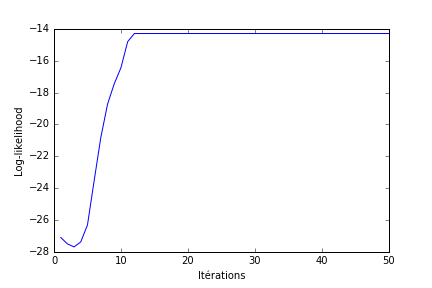
\includegraphics[scale=0.5]{../resources/pictures/M3_K2_hmm.png}
\caption{Évolution de la log-vraisemblance pour inférence exacte \hmm}
\end{figure}
On teste ensuite l'inférence exacte pour le modèle \fhmm.
\begin{figure}[H]
\centering
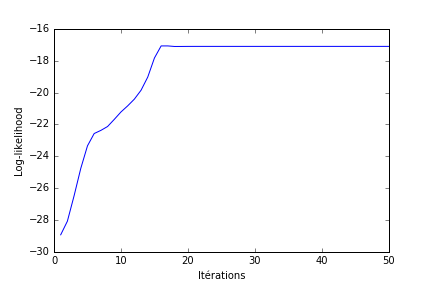
\includegraphics[scale=0.5]{../resources/pictures/M3_K2_fhmm_exact.png}
\caption{Évolution de la log-vraisemblance pour inférence exacte \fhmm}
\end{figure}
Dans les deux cas on observe une stricte croissance de la log-vraisemblance

\subsubsection{Échantillonnage de Gibbs}

Dans \cite{ghahramani1997factorial} les auteurs utilisent l'échantillonnage
de Gibbs en ne considérant pas de période de \textit{burn-in}, aucun
échantillon n'est rejeté.
Les auteurs justifient cette approche par leur volonté de comparer les
approches variationnelles avec un échantillonnage de Gibbs même loin de la
convergence (cet échantillonnage est appelé échantillonnage de Gibbs
impatient).
Les tests d'apprentissage sont toujours effectués avec les mêmes paramètres
aléatoires.
Ici on observe l'évolution de la log-vraisemblance avec l'approche décrite dans
l'article \cite{ghahramani1997factorial}.
L'étape de \textit{burn-in} n'est pas prise en compte et aucun échantillon
n'est rejeté.
Ici le nombre d'échantillons est posé à $N_s=N_r=10$ où $N_r$ est le nombre
d'échantillons créé et $N_s$ le nombre d'échantillons conservé.

\begin{figure}[H]
  \centering
  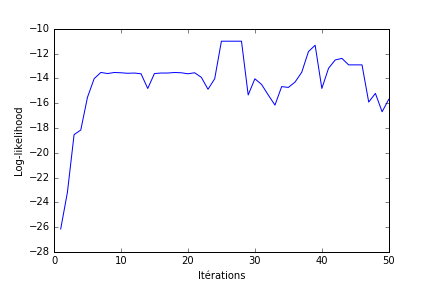
\includegraphics[scale=0.5]{../resources/pictures/M3_K2_gibbsnoburning.png}
  \caption{Évolution de la log-vraisemblance pour l'échantillonneur de Gibbs impatient}
\end{figure}

  Bien qu'on observe une tendance croissante et une stabilisation de la 
log-vraisemblance on conserve une grande variabilité.
Une solution pour tenter d'échantillonner de manière correcte et donc de mieux
vérifier la propriété de croissance est d'introduire du \textit{burn-in} dans
l'échantillonnage de Gibbs.
Ici, on a créé $N_r = 30$ échantillons et on en conserve $N_s = 10$.

\begin{figure}[H]
\centering
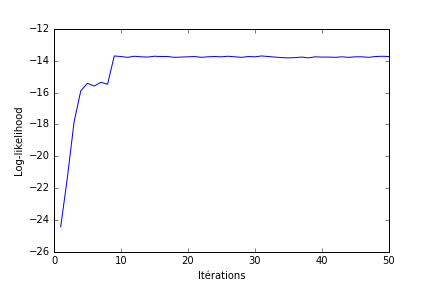
\includegraphics[scale=0.5]{../resources/pictures/M3_K2_gibbs.png}
\caption{Évolution de la log-vraisemblance pour l'échantillonneur de Gibbs}
\end{figure}
On constate que les propriétés de croissance sont meilleures (même si des 
oscillations restent présentes). Néanmoins, on paye cher l'augmentation du 
nombre d'échantillons créés puisque l'algorithme devient bien plus lent que 
l'inférence exacte (avec notre nombre d'états et la taille de l'espace d'états, 
il est évident que si $K$ et $M$ sont plus grands cet échantillonnage restera 
plus rapide que l'inférence exacte). Or le but de l'échantillonnage de Gibbs 
est justement d'éviter d'avoir à passer par une inférence exacte assez lente 
pour des valeurs élevées de $M$ et $K$.
\subsubsection{Approches variationnelles}
Comme décrit précédemment une autre approche du problème consiste à ne pas 
essayer d'échantillonner selon la mesure $p(S_{(t)}^{(m)} \vert Y_{(t)})$ mais 
selon une mesure de probabilité qui s'en approche soumise à des contraintes. La 
contrainte retenue dans le modèle \meanfield{} est l'indépendance entre les 
variables cachées. On rappelle brièvement qu'il convient ensuite de minimiser 
la divergence de Kullback-Lieber entre la probabilité $p(S_{(t)}^{(m)} \vert 
Y_{(t)})$ et les probabilités qui se factorisent dans ce nouveau graphe. La 
minimisation de cette divergence se fait de manière itérative en opérant une 
descente selon chaque coordonnée. Les auteurs de \cite{ghahramani1997factorial} 
remarque que la convergence est très rapide ($N_{it}< 10$ avec $N_{it}$ le 
nombre d'itérations. On observe l'évolution suivante pour la log-vraisemblance 
avec $N_{it} = 5$.

\begin{figure}[H]
\centering
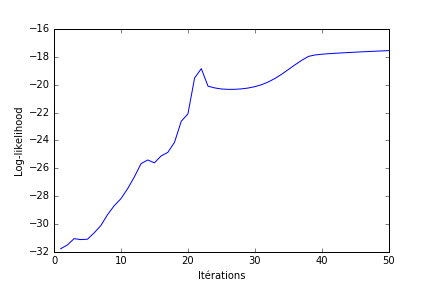
\includegraphics[scale=0.5]{../resources/pictures/M3_K2_meanfield.png}
\caption{Évolution de la log-vraisemblance pour \meanfield}
\end{figure}

Le fait que cette log-vraisemblance ne soit pas strictement croissante est 
justifiée par le fait que la log-vraisemblance est ici une log-vraisemblance 
approchée puisque la mesure de probabilité considérée n'est plus 
$p(S_{(t)}^{(m)} \vert Y_{(t)})$.

On présente également les résultats obtenus pour le modèle \structmeanfield. On rappelle
que l'hypothèse faite sur les états cachés n'est plus une indépendance mais une structure
 de $M$ chaînes de Markov superposées. 
 
 \begin{figure}[H]
\centering
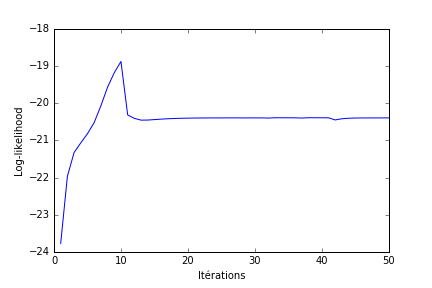
\includegraphics[scale=0.5]{../resources/pictures/M3_K2_structmeanfield.png}
\caption{Évolution de la log-vraisemblance pour \structmeanfield}
\end{figure}
\subsubsection{Comportement aux temps longs}
 Dans les études précédentes ainsi que dans \cite{ghahramani1997factorial} les études sont menées sur de
  courtes chaines ($T=20$). On illustre ici pour le cas $T = 100$ les résultats obtenus via l'inférence 
  exacte.
  
 \begin{figure}[H]
\centering
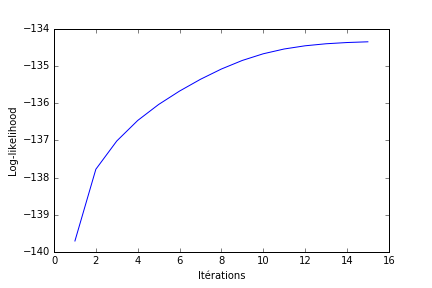
\includegraphics[scale=0.5]{../resources/pictures/M2_K2_T100_exactinference.png}
\caption{$M=2$, $K=2$, $T=100$, inférence exacte}
\end{figure}

Il est à préciser que puisque le nombre de paramètres des modèles variationnels augmente linéairement
avec $T$, il est naturel de devoir augmenter les paramètres itératifs pour s'approcher de la convergence.
Les résultats empiriques obtenus suggèrent que, même pour $T=100$, on observe une stabilisation de la 
log-vraisemblance pour $N_{it}<100$.
\subsection{Un critère : complexité et temps d'exécution}
On a vu dans la partie précédente plusieurs possibilités pour calculer \Estep. Il s'agit maintenant
 d'obtenir des critères pour décider quelle méthode employer. On peut d'abord s'intéresser à la 
 complexité algorithmique de ces méthodes. Ces complexités sont récapitulées dans le tableau suivant.
\newline
\begin{center}
\begin{tabular}{|c|c|}
\hline
Méthode & Complexité algorithmique \\
\hline \hline
\hmm - inférence exacte &  $\mathcal{O}(TK^{2M})$ \\ \hline
\fhmm - inférence exacte &  $\mathcal{O}(TK^{M+1})$ \\ \hline
échantillonnage de Gibbs &  $\mathcal{O}(TKM N_r )$ \\ \hline
\meanfield & $\mathcal{O}(TK^2MN_{it})$ \\ \hline
\structmeanfield & $\mathcal{O}(TK^2MN_{it})$ \\ \hline
\end{tabular}
\end{center}
Dans le tableau suivant on présente les résultats obtenus lors de nos tests sur des modèles génératifs
 avec paramètres d'entrée aléatoires et $M=3$ et $K=2$. On a posé $N_{it}=5$, $N_r=30$ et $N_s=10$. On a toujours $T=10$.
 
\begin{center}
\begin{tabular}{|c|c|}
\hline
Méthode & Temps itération (s) \\
\hline \hline
\hmm - inférence exacte & 0.453  \\ \hline
\fhmm - inférence exacte & 0.429 \\ \hline
échantillonnage de Gibbs &  1.100 \\ \hline
\meanfield & 0.053 \\ \hline
\structmeanfield & 0.319 \\ \hline
\end{tabular}
\end{center}
Ces résultats correspondent à ceux obtenus dans \cite{ghahramani1997factorial}, sauf pour l'inférence
 exacte où \fhmm est plus rapide que \hmm. Néanmoins vu les données de complexité énoncées plus haut il
  semble normal que \fhmm soit plus rapide que \hmm. Il convient aussi de remarquer que les méthodes
   variationnelles possèdent l'avantage de fonctionner même si l'espace d'état est grand. Cela devient
    rapidement faux pour les méthodes d'inférence exacte et pour l'échantillonnage de Gibbs.
 \subsection{Overfitting}
  \bibliographystyle{plain}
  \bibliography{../resources/bibliography/bibfile}
\end{document}